\documentclass{jsbook}

\usepackage[dvipdfmx]{graphicx}
\usepackage{ascmac}
\usepackage{itembkbx}

\begin{document}
\chapter{Paillet6編}
ループを持つ論理回路についてのパートです。\\
自分で学習したものとして詳細な解説は無くして、メモ程度になっています。
部分によっては丁寧に解説しているところもありますが。
\newpage
\section{Paillet6について}
高橋教授の先行研究で中で扱われた回路のうちの1つです。
回路図は図\ref{paillet6}のようになっています。
この回路のモデル化と検証をします。
\begin{figure}[htbp]
\begin{center}
  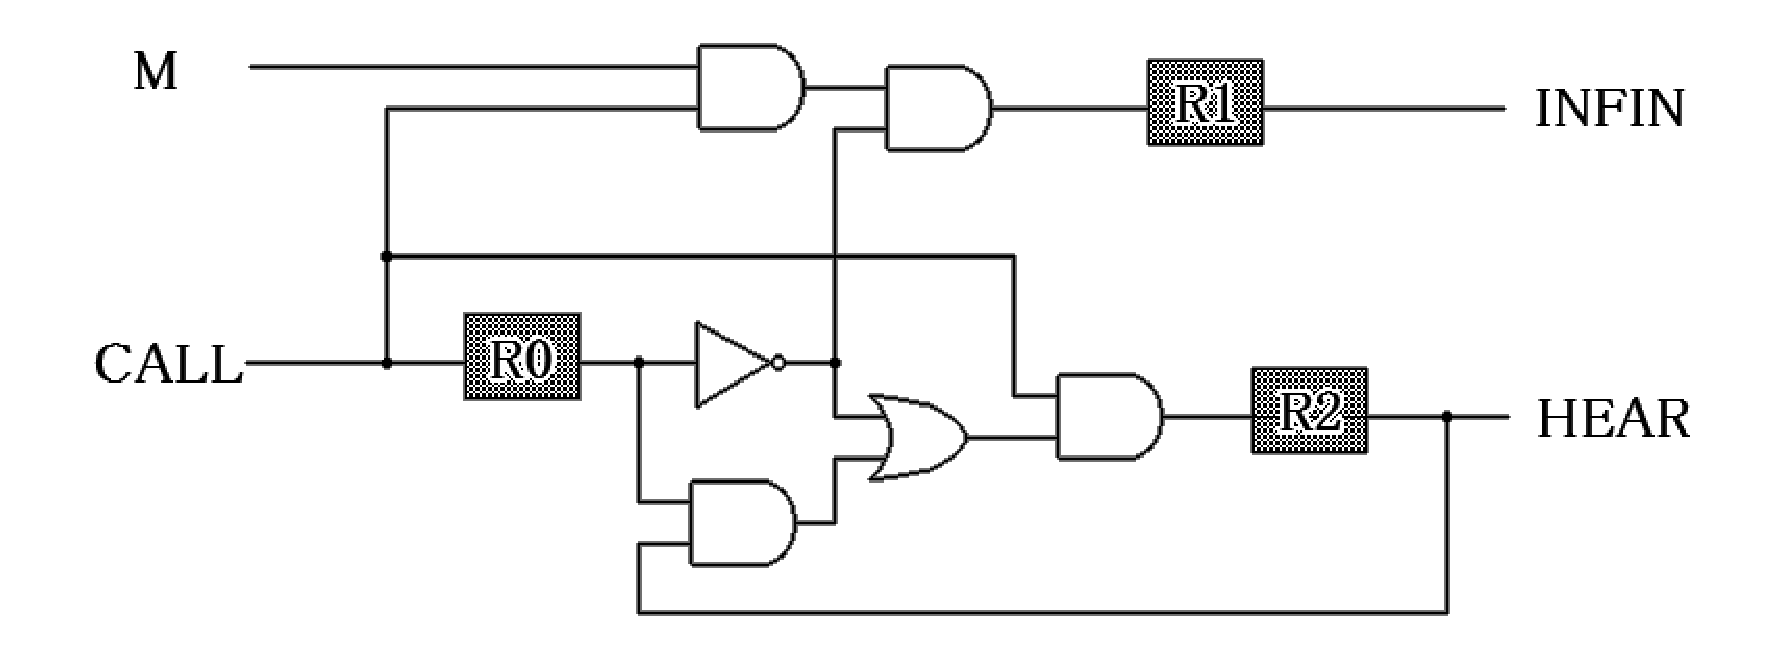
\includegraphics[width=38zw]{image/Paillet6_AE.eps}
  \caption{Paillet6回路}
  \label{paillet6}
\end{center}
\end{figure}

\section{レジスタについて \label{レジスタ}}
加算器と違い、この回路はレジスタを含んでいます。
回路図のR1、R2、R3がそうです。
レジスタには種類がありますが、ここで用いられているレジスタは「入力を1時刻遅らせて出力する」という機能で、いわゆる遅延素子です。
Paillet6の場合は別の実装方法をしていますが、この機能だけを実装したら以下のようになりました。
\begin{verbatim}
Fixpoint delayn(n : nat)(l: list nat): list nat :=
match n with
| 0 => l
| S n' => match l with
          | nil => [0] ++ (delayn n' nil)
          | a::l' => [0] ++ (delayn n' l)
          end
end.
\end{verbatim}
入力の自然数でどれだけ遅延させるかを決め、パターンマッチの中で再帰的に自身を呼び出すことによって複数回遅延を表現しています。
これは自然数 natの場合の遅延ですが、boolの場合でも同様の書き方で定義できます。
変えるべきところは変える必要は当然ありますが。
Paillet6での実装方法はその時に説明します。
\section{Paillet6のモデル化}
基本的には先行研究のモデルを再現するという考えのもと、実装していったのでモデルは先行研究とほぼ同じです。
先行研究ではNQTHMという定理証明器を用いて検証していました。
それをCoq用に書きなおすのが主でした。
しかし、そのままではCoqでは扱えないものがあるので、それは自分で考えながら書き換える必要がありました。

たとえば、natを入力するとboolが出力されるという関数は定義できません。
\begin{verbatim}
Definition test1 (a:nat) : bool := .
\end{verbatim}
と書いた場合は関数の中身を書くことが出来ませんし、
\begin{verbatim}
Definition test2 := nat -> bool.
\end{verbatim}
と書くと、読み込んでくれますが、これを使って別の関数を定義する場合に、型が違うと言われてしまいます。
これ解消するためにDefinitionではなく「Parameter」を使います。
これは関数の中身がかけない代わりに、test2のような書き方で型を合わせることが出来ます。
その代わり、証明モードで展開することが出来ません。
\begin{verbatim}
Parameter test3 = nat -> bool.
\end{verbatim}
と書いて、unfoldしてもnat->boolにはならず、test3のままです。
場合によっては、うまく行かなくなる場合がありますが、今回の場合はかなり内側の、一番展開がされた時にようやく登場するので問題ありません。

また、NQTHM側の都合で単純に処理できていなかったところもCoq用に変更しました。
たとえば、「自然数が0であるかどうかを判定する zerop」という関数や、帰納法を正しく実行させるための「mysub1」などです。
zeropはCoqではパターンマッチで処理できるのでその関数自体を省略しています。
mysub1はNQTHMと違い、$n - 1$を何度繰り返しても、帰納法を用いた時も停止しないことはないので$-1$で記述しています。
そうして書きなおしたモデルが以下になります。

\begin{breakitembox}<parindent = 0zw>[l]{Paillet6のモデル}
  \begin{verbatim}
Definition tau := nat.
Parameter call : tau -> bool.
Parameter m : tau -> bool.

Definition r0_b := call .
Definition r0_a (t:tau) (s0:bool) : bool :=
match t with
| 0 => s0
| S n => r0_b n
end.

Definition r1_b (t:tau)(s0:bool) : bool :=
andb ( andb (m t) (call t)) (negb (r0_a t s0)).
Definition r1_a (t:tau)(s0 s1 : bool) : bool :=
match t with
|0 => s1
|S n => r1_b n s0
end.
Fixpoint r2_a (t:tau)(s0 s2 : bool) : bool :=
match t with
|0 => s2
|S n => andb (call n) 
       (orb (negb (r0_a n s0)) (andb (r0_a n s0) (r2_a n s0 s2)))
end.

Definition infin (t:tau)(s0 s1 : bool) : bool :=
r1_a t s0 s1.

Definition hear (t:tau)(s0 s2 : bool) : bool :=
r2_a t s0 s2.
  \end{verbatim}
\end{breakitembox}
\subsection*{Paillet6のレジスタ}
このモデルにおいてのレジスタはr0\_bからr2\_aまでです。
\ref{レジスタ}節で紹介したレジスタとは違う点がいくつかあり、
\begin{itemize}
\item 入力がリストではない
\item レジスタの前後で定義を分けている
\end{itemize}
などが挙げられます。
まず、「入力がリストではない」ですが、この回路における入力はCALLとMです。
これら2つの入力は「\verb|tau -> bool|」で定義しています。
これは「\emph{nat型の何か}が入力されると\emph{bool型の何か}を出力する」という意味です。
リストは、リストの各要素を時刻とすると各時刻の値が時間によって固定されているのに対し、
この方法は、各時刻の値は不定であるという点が違いです。
2つめの違いは定義どおりを忠実に守ったこと、こうした方が定義が見やすくなるという理由からです。
前後を分けずに一つにまとめても同じように証明できることは確認済みです\footnote{2015/01/23}。
最終的には1つにまとめたものに書き直す予定です。

\section{証明}
この回路が満たすべき性質は以下の二つです。
\begin{itemize}
\item{INFINがtrueとなるのは1時刻前のMおよびCALLがtrueで2時刻前のCALLがfalseの場合でありかつそのときに限る}
$$\mbox{INFIN}(\tau)=\mbox{M}(\tau-1) \wedge \mbox{CALL}(\tau-1) \wedge \lnot \mbox{CALL}(\tau-2)$$
\item{HEARがtrueになるのは1時刻前のCALLがtrueの場合でかつそのときに限る}
$$\mbox{HEAR}(\tau) = \mbox{CALL}(\tau-1)$$
※レジスタの初期値はs0,s2ともにfalseであると仮定
\end{itemize}
ここで$\tau$は時刻を示します。
これらを証明しました。
モデル化が終わった時にこれをそのまま証明しようとしてみたのですが、いろいろな問題を見落としていたため証明はできませんでした。

まず、証明ができなかった理由として、$\tau-1$や$\tau-2$を見落としていたことです。
今回、時間を自然数で定義しているため、いくらマイナスを重ねても0より下に下がることはありません。
そのため、$\tau$が1以下の場合に正しい性質を満たせなくなります。
したがって、$\tau > 1$という前提条件を追加しました。

前提条件以外はすべて上記の性質を、定義したものを使ってそのまま書き下してLammaを書きました。

\begin{itembox}[l]{Lemma}
\begin{verbatim}
Lemma infin_is_correct : forall (t:tau)(s0 s1:bool), 
t>1 ->
(infin t s0 s1 = 
andb ( andb ( m (t-1)) (call (t-1))) (negb ( call ((t-2))))).

Lemma hear_is_correct : forall (t:tau)(s0 s2:bool),
(s0 = false /\ s2 = false) -> t > 0 ->
(hear t s0 s2 = call (t-1)).
\end{verbatim}
\end{itembox}

\subsection*{INFINの証明}
前述の通りINFINは$\tau$が2以上の場合のみに成り立ちます。
そのため、destructタクティックを用いて場合分けを行います。
最初はinductionを使って場合分けをしていたのですが、ループがないためinductionを使う必要はありませんでした。
場合分けをすると、\verb|0>1|などの明らかに間違った仮定が現れます。
それらをinversionタクティックを使って除外します。
これで1以下の場合の証明は終了です。

次に2以上の場合の証明です。
まずは単純化をして、そこから方向性を決めていきます。
仮定に適用出来そうなものはなく、展開できそうなものが多いので展開していきます。
まずr1\_bから展開すると、両辺が同じような形になったので、この方向性で証明できそうな気がしてきました。
展開した左辺にr0\_aが出てきて、これも展開できるので展開して、次に出てくるbも展開すると\verb|t -0|がある以外は等しくなりました。
単純化してもこれを\verb|t|にはしてくれないので、ライブラリから0を消せるタクティックを探して適用しました。
すると両辺が等しくなり、reflexivityを使えるのでこれで証明できました。

\subsection*{HEARの証明}
HEARの場合はループがあるので、INFINで使わなかったinductionが必要になりました。
途中まではINFINと同じような感じで、ただし、inductionを使って$\tau = 0$の場合を除外します。
そして、INFINの2以上の場合と同じように証明を進めたいのですがループがあるため上手く行きません。
これは展開を進めていくとパターンマッチ文が出てくるためです。
出てくるパターンマッチはtに関するものなのでtについて場合分けしました。
その後単純化した式にレジスタの初期値を代入すると式が簡単になりそうなので代入します。
代入すると非常に簡単な式になったのですが、これも単純化出来ないためcall 0について場合分けをして証明しました。

最後のサブゴールを単純化すると非常にごちゃごちゃした式になってしまいました。
最初はここからどうすれば良いのか分からず、繰り返して今までの証明をくり返していました。
どうしようもなくなってしまったのでポスドクの方に尋ねると、仮定も簡略化するとサブゴールに仮定を使える部分が出てくると教えてくださいました。
教えて頂いたとおりに簡略化し、両方を見比べてみると同じ部分があり、その部分を仮定で書き換えを行いました。
そうするとかなりシンプルな形になました。
式を見ると、\verb|call tと call (S t)|ばかりなので、これらについて場合分けを行いそれぞれ証明進めました。
最後に、書き換えをした際に出てきたゴールが1つ残ったのですが、これは仮定の$t>0$が出てきたので、これを証明したLemmaをライブラリから探して適用してHEARの証明は完了しました。


\end{document}